%
% Projekt: proj5.tex
% Autor:   Michal Ľaš
% Datum:   19.04.2023
% 


\documentclass{beamer}
\usetheme{Antibes}
\usepackage[slovak]{babel}
\usepackage{times}
\usepackage[utf8]{inputenc}
\usepackage{graphicx}
\usepackage[ruled, slovak, linesnumbered, noline, longend]{algorithm2e}
\usepackage{tikz}
\usetikzlibrary{positioning}


% pridať číslovanie snímkov
\setbeamertemplate{footline}
{
  \hbox
  {
	\begin{beamercolorbox}[wd=1\paperwidth,ht=2.25ex,dp=1ex,right]{framenumber}
    	\usebeamerfont{framenumber}\insertframenumber{} / \inserttotalframenumber\hspace*{2ex}
    \end{beamercolorbox}}
  \vskip 2pt
}
% odstrániť navigáciu
\setbeamertemplate{navigation symbols}{}

%%%%%%%%%%%%%%%%%%%% Počítadlo snímkov v sekcii %%%%%%%%%%%%%%%%%%%%

% Vytvoríme nový počítadlo pre snímky v sekcii
\newcounter{sectionslides}

% Resetujeme počítadlo na začiatku každej sekcie
\AtBeginSection[]{
  \setcounter{sectionslides}{0}
}

% Zvýšime počítadlo pre každý snímok
\AtBeginEnvironment{frame}{
  \ifnum\value{sectionslides}=0
    \setcounter{sectionslides}{1}
  \else
    \stepcounter{sectionslides}
  \fi
}

% Príkaz pre zobrazenie počítadla snímok v sekcii
\newcommand{\sectionslidenumber}{
  (\thesectionslides/\the\numexpr\insertsectionendpage-\insertsectionstartpage+1\relax)
}

%%%%%%%%%%%%%%%%%%%%%%%%%%%%%%%%%%%%%%%%%%%%%%%%%%%%%%%%%%%%%%%%%%%%


\title{Typografie a~publikování\,--\,5.~projekt}
\subtitle{Grafové algoritmy\,--\,Dijkstrov algoritmus}
\author{\texorpdfstring{Michal Ľaš\newline\url{xlasmi00@stud.fit.vutbr.cz}}{Michal Ľaš}}
\institute
{
	Vysoké učení technické v~Brně\\
	Fakulta informačních technologií
}
\date{\today}


\begin{document}

\frame{\titlepage}

%%% Osnova %%%
\section{Prehľad}

\begin{frame}{\insertsectionhead}
	\tableofcontents
\end{frame}

%%% Kto bol Dijkstra %%%
\section{Edsger Wybe Dijkstra}

\begin{frame}[c]{\insertsectionhead~(11. máj 1930\,--\,6. august 2002)}
	\begin{columns}[T]
		\begin{column}{0.5\textwidth}
			\begin{figure}
				\centering
				\scalebox{0.32}{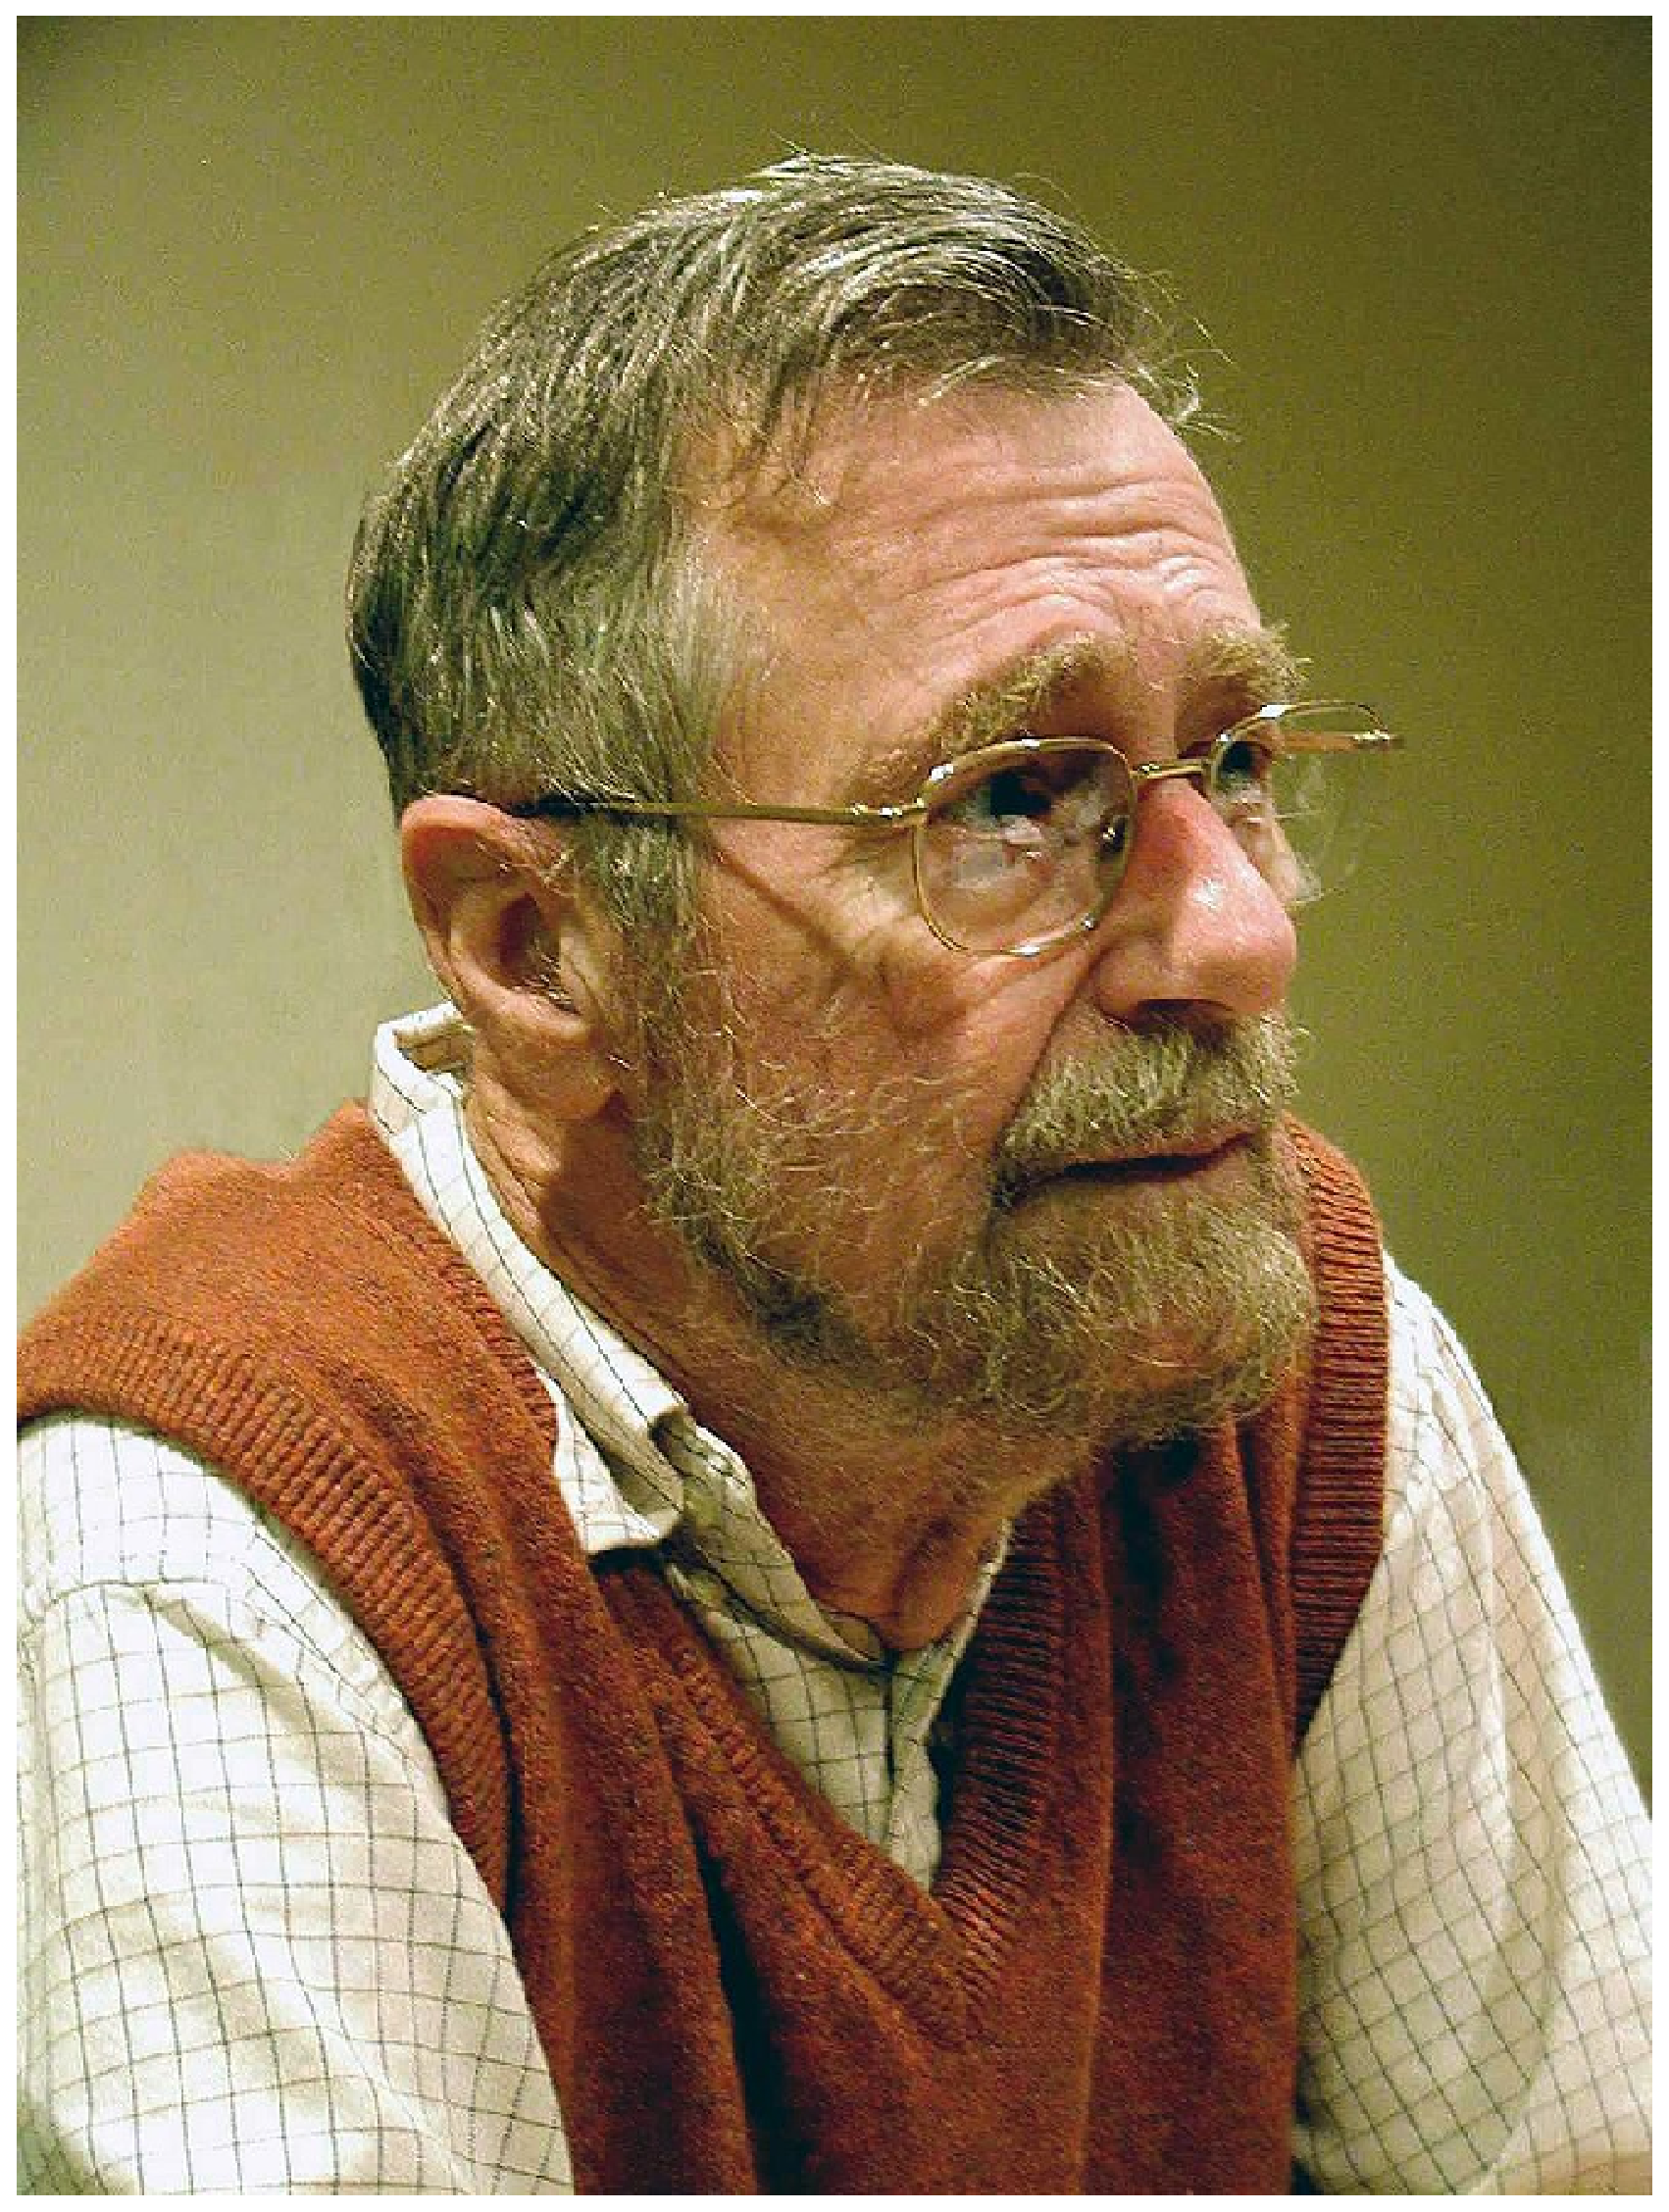
\includegraphics[scale=0.5]{obrazky/Dijkstra.eps}}
			\end{figure}
		\end{column}

		\begin{column}{0.5\textwidth}
			\begin{itemize}
				\vspace{12pt}
				\setlength{\itemsep}{12pt}
				\item Holandský informatik
				\item Držiteľ Turingovej ceny (1972)
				\item idea semaforu 
				\item nástroje pre synchronizáciu viacerých procesov
				\item algoritmus pre nájdenie najkratšej cesty v~grafe
			\end{itemize}
		\end{column}
	\end{columns}
\end{frame}


%%% Algoritmus %%%
\section{Dijkstrov algoritmus}

\begin{frame}{{\insertsectionhead\sectionslidenumber}}
	Algoritmus na nájdenie najkratšej cesty v~grafe
	
	\begin{block}{popis}
		Majme ohodnotený hraf $G$ v ktorom hľadáme najkratšiu cestu.

		\begin{itemize}
			\item $V$ je množina všetkých vrcholov grafu $G$
			\item $E$ je množina, ktorá obsahuje všetky hrany grafu $G$
			\item Dĺžka najkratšej cesty do vrchlu $v \in V$ je označená ako $d[v]$
			\item $Z \subseteq V$ je množina, ktorá obsahuje navštívené vrcholy
			\item $N \subseteq V$ je množina, doposiaľ nenavštívených vrcholov
		\end{itemize}

		Na začiatku majú všetky vrcholy hodnotu $d[v] := \infty$ okrem počiatočného bodu $s \in V$, kde $d[s] := 0$.
	\end{block}
\end{frame}


\begin{frame}{Pseudokód\sectionslidenumber}
	\footnotesize
	\IncMargin{1.5em}
	\begin{algorithm}[H]
		\ForEach{$v$ in $V$}
		{
			$d[v] := \infty$\\
			$\pi[v] := None$\\ 
		}
		$d[s] := 0$\\
		$Z := \varnothing$\\
		$N := V$\\
		\While{$N \neq \varnothing$}
		{
			$u := $ extract-min$(N)$; $Z.add(u)$\\
			\ForEach{$v$ in $u$}{
				\uIf{$d[v] > d[u] + l(u,v)$}{
					$d[v] := d[u] + l(u,v)$\\
					$\pi[v] := u$\\
				}
			}
		}
		\Return{$ X_t $}
	
		\caption{\textsc{Dijkstrov algoritmus}}
		\label{algorithm:dijkstra}
	\end{algorithm}
	\DecMargin{1.5em}
	\normalsize
\end{frame}


\section{Demonštrácia}

\begin{frame}{\insertsectionhead}
	\begin{center}
		\begin{tikzpicture}[
			roundnode/.style={circle, draw=blue!60, fill=blue!5, very thick, minimum size=12mm},
			path/.style={very thick}
		]
			\node[roundnode](point_s){s/0};
			\node[roundnode](point_a)[below left=of point_s]{a/$\infty$};
			\node[roundnode](point_b)[below right=of point_s]{b/$\infty$};
			\node[roundnode](point_c)[below=of point_a]{c/$\infty$};
			\node[roundnode](point_d)[below=of point_b]{d/$\infty$};

			\draw[->, line width=1] (point_s.west) -- node[above, draw=none]{4} (point_a.north);
			\draw[->, line width=1] (point_s.east) -- node[above, draw=none]{12} (point_b.north);
			\draw[->, line width=1] (point_a.east) -- node[above, draw=none]{5} (point_b.west);
			\draw[->, line width=1] (point_a.south) -- node[left, draw=none]{4} (point_c.north);
			\draw[->, line width=1] (point_a.south east) -- node[above, draw=none]{8} (point_d.north west);
			\draw[->, line width=1] (point_b.south) -- node[right, draw=none]{1} (point_d.north);
			\draw[->, line width=1] (point_c.east) -- node[below, draw=none]{3} (point_d.west);

			\pause
			\node[roundnode,draw=red,fill=red!60](point_s){s/0};
			\node[roundnode](point_a)[below left=of point_s]{a/4};
			\node[roundnode](point_b)[below right=of point_s]{b/12};
			\draw[->, line width=1, red] (point_s.west) -- node[above, draw=none, black]{4} (point_a.north);
			\draw[->, line width=1, red] (point_s.east) -- node[above, draw=none, black]{12} (point_b.north);
			\pause
			\draw[->, line width=1, black] (point_s.east) -- node[above, draw=none, black]{12} (point_b.north);
			\node[roundnode,draw=red,fill=red!60](point_a)[below left=of point_s]{a/4};
			\node[roundnode](point_b)[below right=of point_s]{b/9};
			\node[roundnode](point_c)[below=of point_a]{c/8};
			\node[roundnode](point_d)[below=of point_b]{d/12};
			\draw[->, line width=1,red] (point_a.east) -- node[above, draw=none,black]{5} (point_b.west);
			\draw[->, line width=1,red] (point_a.south) -- node[left, draw=none,black]{4} (point_c.north);
			\draw[->, line width=1,red] (point_a.south east) -- node[above, draw=none, black]{8} (point_d.north west);
			\pause
			\draw[->, line width=1,black] (point_a.south east) -- node[above, draw=none, black]{8} (point_d.north west);
			\node[roundnode,draw=red,fill=red!60](point_c)[below=of point_a]{c/8};
			\draw[->, line width=1,red] (point_c.east) -- node[below, draw=none,black]{3} (point_d.west);
			\node[roundnode](point_d)[below=of point_b]{d/11};
			\pause
			\draw[->, line width=1,black] (point_c.east) -- node[below, draw=none,black]{3} (point_d.west);
			\node[roundnode,draw=red,fill=red!60](point_b)[below right=of point_s]{b/9};
			\draw[->, line width=1,red] (point_b.south) -- node[right, draw=none,black]{1} (point_d.north);
			\node[roundnode](point_d)[below=of point_b]{d/10};
			\pause
			\node[roundnode,draw=red,fill=red!60](point_d)[below=of point_b]{d/10};



		\end{tikzpicture}
	\end{center}
\end{frame}


%%% Zhrnutie %%%
\section{Zhrnutie}

\begin{frame}{\insertsectionhead}
	Časová náročnosť algoritmu je $O(|V|^2+|E|)$, kde $V$ je počet vrcholov a $E$ je počet hrán.\\
	\vspace{16pt}
	Algoritmus je však možné optimalizovať pomocou binárnej či Fibonačiho haldy. V tomto prípade by bola zložitosť $O(|E|+|V|log|V|)$.
\end{frame}


%%% Zdroje %%%
\section*{Zdroje}

\begin{frame}{\insertsectionhead}
	Edsger Wybe Dijkstra\\ \indent\footnotesize\url{https://sk.wikipedia.org/wiki/Edsger_Wybe_Dijkstra}\normalsize\\
	Dijkstrův algoritmus\\ \indent\footnotesize\url{https://cs.wikipedia.org/wiki/Dijkstruv_algoritmus}\normalsize\\
\end{frame}


\end{document}